\documentclass{article}

\usepackage{fancyhdr} % Required for custom headers
\usepackage{lastpage} % Required to determine the last page for the footer
\usepackage{extramarks} % Required for headers and footers
\usepackage[usenames,dvipsnames]{color} % Required for custom colors
\usepackage{graphicx} % Required to insert images
\usepackage{listings} % Required for insertion of code
\usepackage{courier} % Required for the courier font
\usepackage{lipsum} % Used for inserting dummy 'Lorem ipsum' text into the template
\usepackage{amsmath}
\usepackage{amssymb}
\usepackage{mathtools, xparse}
\usepackage{booktabs}
\usepackage{bigstrut}
\usepackage{float}
\usepackage{hyperref}
\usepackage{color}
\usepackage{algorithm}
\usepackage{caption}
\usepackage{algpseudocode}
\usepackage{multirow}
\usepackage{subfigure}

\DeclarePairedDelimiter{\norm}{\lVert}{\rVert}
\DeclarePairedDelimiter\abs{\lvert}{\rvert}%

\hypersetup{
    colorlinks   = true,    % Colours links instead of ugly boxes
    urlcolor     = red,    % Colour for external hyperlinks
    linkcolor    = red,    % Colour of internal links
    citecolor    = red      % Colour of citations
}
% Margins
\topmargin=-0.45in
\evensidemargin=0in
\oddsidemargin=0in
\textwidth=6.5in
\textheight=9.0in
\headsep=0.25in

\linespread{1.1} % Line spacing

% Set up the header and footer
\pagestyle{fancy}
\lhead{\hmwkAuthorName} % Top left header
\chead{\hmwkClass\ : \hmwkID} % Top center head
\rhead{\firstxmark} % Top right header
\lfoot{\lastxmark} % Bottom left footer
\cfoot{} % Bottom center footer
\rfoot{Page\ \thepage\ of\ \protect\pageref*{LastPage}} % Bottom right footer
\renewcommand\headrulewidth{0.4pt} % Size of the header rule
\renewcommand\footrulewidth{0.4pt} % Size of the footer rule

\setlength\parindent{0pt} % Removes all indentation from paragraphs

%----------------------------------------------------------------------------------------
%	CODE INCLUSION CONFIGURATION
%----------------------------------------------------------------------------------------

\definecolor{MyDarkGreen}{rgb}{0.0,0.4,0.0} % This is the color used for comments
\lstloadlanguages{Perl} % Load Perl syntax for listings, for a list of other languages supported see: ftp://ftp.tex.ac.uk/tex-archive/macros/latex/contrib/listings/listings.pdf
\lstset{language=Perl, % Use Perl in this example
    frame=single, % Single frame around code
    basicstyle=\small\ttfamily, % Use small true type font
    keywordstyle=[1]\color{Blue}\bf, % Perl functions bold and blue
    keywordstyle=[2]\color{Purple}, % Perl function arguments purple
    keywordstyle=[3]\color{Blue}\underbar, % Custom functions underlined and blue
    identifierstyle=, % Nothing special about identifiers                                         
    commentstyle=\usefont{T1}{pcr}{m}{sl}\color{MyDarkGreen}\small, % Comments small dark green courier font
    stringstyle=\color{Purple}, % Strings are purple
    showstringspaces=false, % Don't put marks in string spaces
    tabsize=5, % 5 spaces per tab
    %
    % Put standard Perl functions not included in the default language here
    morekeywords={rand},
    %
    % Put Perl function parameters here
    morekeywords=[2]{on, off, interp},
    %
    % Put user defined functions here
    morekeywords=[3]{test},
    %
    morecomment=[l][\color{Blue}]{...}, % Line continuation (...) like blue comment
    numbers=left, % Line numbers on left
    firstnumber=1, % Line numbers start with line 1
    numberstyle=\tiny\color{Blue}, % Line numbers are blue and small
    stepnumber=5 % Line numbers go in steps of 5
}

% Creates a new command to include a perl script, the first parameter is the filename of the script (without .pl), the second parameter is the caption
\newcommand{\perlscript}[2]{
    \begin{itemize}
        \item[]\lstinputlisting[caption=#2,label=#1]{#1.py}
    \end{itemize}
}
\newcommand{\cppscript}[1]{
    \begin{itemize}
        \item[]\lstinputlisting[]{#1}
    \end{itemize}
}

%----------------------------------------------------------------------------------------
%	DOCUMENT STRUCTURE COMMANDS
%	Skip this unless you know what you're doing
%----------------------------------------------------------------------------------------

% Header and footer for when a page split occurs within a problem environment
\newcommand{\enterProblemHeader}[1]{
    \nobreak\extramarks{#1}{#1 continued on next page\ldots}\nobreak
    \nobreak\extramarks{#1 (continued)}{#1 continued on next page\ldots}\nobreak
}

% Header and footer for when a page split occurs between problem environments
\newcommand{\exitProblemHeader}[1]{
    \nobreak\extramarks{#1 (continued)}{#1 continued on next page\ldots}\nobreak
    \nobreak\extramarks{#1}{}\nobreak
}

%\setcounter{secnumdepth}{0} % Removes default section numbers
\newcounter{homeworkProblemCounter} % Creates a counter to keep track of the number of problems

\newcommand{\homeworkProblemName}{}
\newenvironment{homeworkProblem}[1][Problem \arabic{homeworkProblemCounter}]{ % Makes a new environment called homeworkProblem which takes 1 argument (custom name) but the default is "Problem #"
    \stepcounter{homeworkProblemCounter} % Increase counter for number of problems
    \renewcommand{\homeworkProblemName}{#1} % Assign \homeworkProblemName the name of the problem
    \section{\homeworkProblemName} % Make a section in the document with the custom problem count
    \enterProblemHeader{\homeworkProblemName} % Header and footer within the environment
    }{
    \exitProblemHeader{\homeworkProblemName} % Header and footer after the environment
}

\newcommand{\problemAnswer}[1]{ % Defines the problem answer command with the content as the only argument
\noindent\framebox[\columnwidth][c]{\begin{minipage}{0.98\columnwidth}#1\end{minipage}} % Makes the box around the problem answer and puts the content inside
}

\newcommand{\homeworkSectionName}{}
\newenvironment{homeworkSection}[1]{ % New environment for sections within homework problems, takes 1 argument - the name of the section
    \renewcommand{\homeworkSectionName}{#1} % Assign \homeworkSectionName to the name of the section from the environment argument
    \subsection{\homeworkSectionName} % Make a subsection with the custom name of the subsection
    \enterProblemHeader{\homeworkProblemName\ [\homeworkSectionName]} % Header and footer within the environment
    }{
    \enterProblemHeader{\homeworkProblemName} % Header and footer after the environment
}

%----------------------------------------------------------------------------------------
%	NAME AND CLASS SECTION
%----------------------------------------------------------------------------------------

\newcommand{\hmwkID}{homework 10} % Assignment title
\newcommand{\hmwkTitle}{Numerical Integration}
\newcommand{\hmwkDueDate}{Tuesday,\ May\ 9,\ 2017} % Due date
\newcommand{\hmwkClass}{Numerical Analysis} % Course/class
\newcommand{\hmwkClassTime}{10:30am} % Class/lecture time
\newcommand{\hmwkClassInstructor}{Jones} % Teacher/lecturer
\newcommand{\hmwkAuthorName}{102061149 Fu-En Wang} % Your name

%----------------------------------------------------------------------------------------
%	TITLE PAGE
%----------------------------------------------------------------------------------------

\title{
    \vspace{2in}
    \textmd{\textbf{\hmwkClass}}\\
    \textmd{\textbf{\hmwkID: \hmwkTitle}} \\
    \normalsize\vspace{0.1in}\small{Due\ on\ \hmwkDueDate}\\
    \vspace{3in}
}

\author{\textbf{\hmwkAuthorName}}
\date{} % Insert date here if you want it to appear below your name

%----------------------------------------------------------------------------------------

\begin{document}
\maketitle
\newpage

\section{Introduction}
\label{sec:intro}
In this assignment, we will implement Newton-Cotes Integration to calculate the following function:
\begin{align}
    & f(x) = e^x \\
    & I = \int_0^2f(x)dx
\end{align}
Because the integration of $e^x$ can be evaluated by ourself, so we have the groundtruth:
\begin{align}
    I^* = e^2 - e^0 \approx 6.389056
\end{align}
We will divide the interval 0 to 2 into 12, 24, 96, 192, 384, 768, 1536 subintervals, respectively, and calculate the error with different
order. For 12 subintervals, we will create 13-vector X and Y:
\begin{align*}
    & h = \frac{2}{12} \\
    & X[k] = k * h \\
    & Y[k] = e^{X[k]}
\end{align*}
X, Y and order will be our input parameter of function.

\section{Implementation}
\begin{algorithm}[H]
    \caption{\textbf{Newton-Cotes Integration}}
    \begin{algorithmic}
        \State Input is order, VEC X, VEC Y
        \State len = size of X
        \State $W$ is weight of the order.
        \State sum = 0
        \For{each i $\in$ \{0, order, 2$*$order, 3$*$order, ...., len-2\}}
            \For{each k $\in$ \{0, 1, 2, ..., order\}}
                \State sum += W[k] * Y[i+k]
            \EndFor
        \EndFor
        \State \textbf{return} sum * (X[1] - X[0])
    \end{algorithmic}
\end{algorithm}

\section{Discussion}
From Section \ref{sec:intro}, we have already known that:
$$
    I^* \approx 6.389056
$$
As a result, we will calculate the error with different subintervals and order in this section.
\subsection{Experiment Result}
For convinient purpose, I will refer $I_k^n$ and $E_k^n$ as my answer and error with k subintervals and order n, respectively. \newline
The following tables show the experiment result.

\begin{table}[H]
    \centering 
    \caption{Experiment Result}
    \label{tab:all}
    \subtable[Result of 12 subintervals]{
        \begin{tabular}{|c|c|c|c|}
            \hline
            $I_{12}^1$ & 6.403839 & $E_{12}^1$ & 1.48E-02 \\ \hline
            $I_{12}^2$ & 6.389083 & $E_{12}^2$ & 2.73E-05 \\ \hline
            $I_{12}^3$ & 6.389117 & $E_{12}^3$ & 6.12E-05 \\ \hline
            $I_{12}^4$ & 6.389056 & $E_{12}^4$ & 2.86E-07 \\ \hline
            $I_{12}^6$ & 6.389056 & $E_{12}^6$ & 3.94E-09 \\ \hline
        \end{tabular}
        \label{tab:12}
    }
    \subtable[Result of 24 subintervals]{
        \begin{tabular}{|c|c|c|c|}
            \hline
            $I_{24}^1$ & 6.392753 & $E_{24}^1$ & 3.70E-03 \\ \hline
            $I_{24}^2$ & 6.389058 & $E_{24}^2$ & 1.71E-06 \\ \hline
            $I_{24}^3$ & 6.38906 & $E_{24}^3$ & 3.85E-06 \\ \hline
            $I_{24}^4$ & 6.389056 & $E_{24}^4$ & 4.51E-09 \\ \hline
            $I_{24}^6$ & 6.389056 & $E_{24}^6$ & 1.58E-11 \\ \hline
        \end{tabular}
        \label{tab:24}
    }
    \subtable[Result of 48 subintervals]{
        \begin{tabular}{|c|c|c|c|}
            \hline
            $I_{48}^1$ & 6.38998 & $E_{48}^1$ & 9.24E-04 \\ \hline
            $I_{48}^2$ & 6.389056 & $E_{48}^2$ & 1.07E-07 \\ \hline
            $I_{48}^3$ & 6.389056 & $E_{48}^3$ & 2.41E-07 \\ \hline
            $I_{48}^4$ & 6.389056 & $E_{48}^4$ & 7.07E-11 \\ \hline
            $I_{48}^6$ & 6.389056 & $E_{48}^6$ & 6.04E-14 \\ \hline
        \end{tabular}
        \label{tab:48}
    }
    \subtable[Result of 96 subintervals]{
        \begin{tabular}{|c|c|c|c|}
            \hline
            $I_{96}^1$ & 6.389287 & $E_{96}^1$ & 2.31E-04 \\ \hline
            $I_{96}^2$ & 6.389056 & $E_{96}^2$ & 6.69E-09 \\ \hline
            $I_{96}^3$ & 6.389056 & $E_{96}^3$ & 1.50E-08 \\ \hline
            $I_{96}^4$ & 6.389056 & $E_{96}^4$ & 1.10E-12 \\ \hline
            $I_{96}^6$ & 6.389056 & $E_{96}^6$ & 0 \\ \hline
        \end{tabular}
        \label{tab:96}
    }
    \subtable[Result of 192 subintervals]{
        \begin{tabular}{|c|c|c|c|}
            \hline
            $I_{192}^1$ & 6.389114 & $E_{192}^1$ & 5.78E-05 \\ \hline
            $I_{192}^2$ & 6.389056 & $E_{192}^2$ & 4.18E-10 \\ \hline
            $I_{192}^3$ & 6.389056 & $E_{192}^3$ & 9.40E-10 \\ \hline
            $I_{192}^4$ & 6.389056 & $E_{192}^4$ & 1.69E-14 \\ \hline
            $I_{192}^6$ & 6.389056 & $E_{192}^6$ & 1.78E-15 \\ \hline
        \end{tabular}
        \label{tab:192}
    }
    \subtable[Result of 384 subintervals]{
        \begin{tabular}{|c|c|c|c|}
            \hline
            $I_{384}^1$ & 6.389071 & $E_{384}^1$ & 1.44E-05 \\ \hline
            $I_{384}^2$ & 6.389056 & $E_{384}^2$ & 2.61E-11 \\ \hline
            $I_{384}^3$ & 6.389056 & $E_{384}^3$ & 5.88E-11 \\ \hline
            $I_{384}^4$ & 6.389056 & $E_{384}^4$ & 3.55E-15 \\ \hline
            $I_{384}^6$ & 6.389056 & $E_{384}^6$ & 8.88E-16 \\ \hline
        \end{tabular}
        \label{tab:384}
    }
    \subtable[Result of 768 subintervals]{
        \begin{tabular}{|c|c|c|c|}
            \hline
            $I_{768}^1$ & 6.38906 & $E_{768}^1$ & 3.61E-06 \\ \hline
            $I_{768}^2$ & 6.389056 & $E_{768}^2$ & 1.64E-12 \\ \hline
            $I_{768}^3$ & 6.389056 & $E_{768}^3$ & 3.66E-12 \\ \hline
            $I_{768}^4$ & 6.389056 & $E_{768}^4$ & 0 \\ \hline
            $I_{768}^6$ & 6.389056 & $E_{768}^6$ & 1.78E-15 \\ \hline
        \end{tabular}
        \label{tab:768}
    }
    \subtable[Result of 1536 subintervals]{
        \begin{tabular}{|c|c|c|c|}
            \hline
            $I_{1536}^1$ & 6.389057 & $E_{1536}^1$ & 9.03E-07 \\ \hline
            $I_{1536}^2$ & 6.389056 & $E_{1536}^2$ & 1.07E-13 \\ \hline
            $I_{1536}^3$ & 6.389056 & $E_{1536}^3$ & 2.27E-13 \\ \hline
            $I_{1536}^4$ & 6.389056 & $E_{1536}^4$ & 8.88E-16 \\ \hline
            $I_{1536}^6$ & 6.389056 & $E_{1536}^6$ & 7.99E-15 \\ \hline
        \end{tabular}
        \label{tab:1536}
    }
\end{table}
From Table \ref{tab:all}, we can plot Error vs Different Order as shown in Figure \ref{fig:error_order}.
\begin{figure}[H]
    \centering
    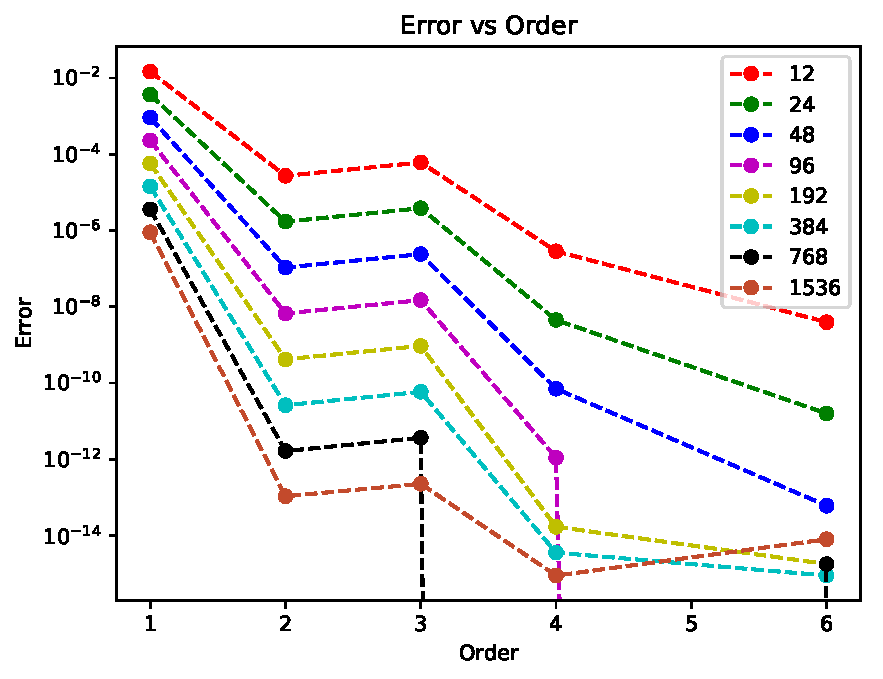
\includegraphics[width=0.6\textwidth]{src/error.pdf}
    \caption{Error vs Order}
    \label{fig:error_order}
\end{figure}
In Figure \ref{fig:error_order}, we can find that 2-order and 3-order are very close and 3-order have a higher error than 2-order. In addition, 
because $E_{96}^6$ and $E_{768}^4$ become 0, so the figure is cut at the two position. To analyze the error more clearly, we can 
plot Error vs number of subintervals as shown in Figure \ref{fig:error_int}
\begin{figure}[H]
    \centering
    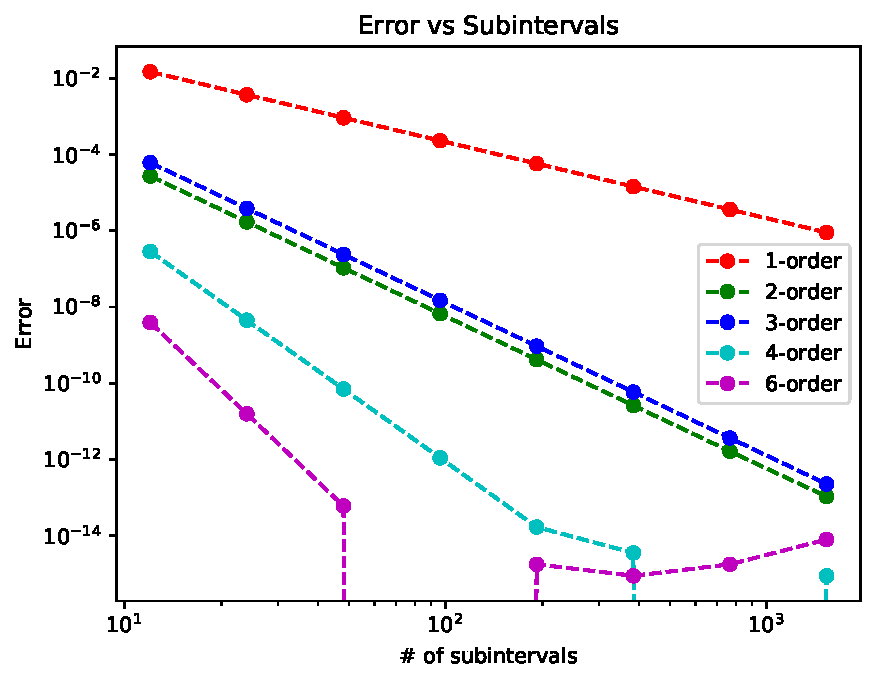
\includegraphics[width=0.6\textwidth]{src/error2.pdf}
    \caption{Error vs Subintervals}
    \label{fig:error_int}
\end{figure}
We can see that 2-order and 3-order are indeed very close. The reason lies on \textbf{Theorem 6.1.5} in class material.
\begin{align}
    & E_{n, m}(f) = \frac{b-a}{(n+2)!}\frac{H^{n+2}}{n^{n+3}}f^{n+2}(\xi)\int_0^nt\prod_{i=0}^n(t-i)dt\text{, if n is even}. \\
    & E_{n, m}(f) = \frac{b-a}{(n+1)!}\frac{H^{n+1}}{n^{n+2}}f^{n+1}(\xi)\int_0^n\prod_{i=0}^n(t-i)dt\text{, if n is odd}.
\end{align}
From this Theorem, we can found that the error of pair [0-order, 1-order], [2-order, 3-order], [4-order, 5-order] 
and [6-order, 7-order] should be close. However, in our case we only have [2-order, 3-order] and they are close in Figure \ref{fig:error_int},
which satisfies the \textbf{Theorem 6.1.5}.

Another strange phenomenon is that 6-order will get larger error after more that 384 subintervals. I think this is because we use 
\textbf{double type} to calculate the data, but double precision number will have \textbf{larger error} after $10^{-15}$. In other words,
the step size is too small for double precision. Maybe we can fix this problem if we use \textbf{long double}.
\end{document}













